\documentclass[conference,a4paper]{IEEEtran}

% Vietnamese support (pdfLaTeX / Overleaf)
\usepackage[utf8]{inputenc}
\usepackage[T5]{fontenc}
\usepackage[vietnamese]{babel}

% Conference typography and layout
\usepackage{lmodern}
\usepackage{microtype}
\usepackage{cite}
\usepackage{graphicx}
\usepackage{booktabs}
\usepackage{tabularx}
\usepackage{array}
\usepackage{amsmath}
% IEEEtran handles conference captions natively.
\usepackage{enumitem}
\usepackage{url}
\usepackage[hidelinks]{hyperref}

% Compact, consistent captions and lists
\setlist{nosep,leftmargin=*}
\renewcommand{\arraystretch}{1.05}
\emergencystretch=1em

\title{Phân loại chủ đề tin tức BBC News bằng TF-IDF và biểu diễn BERT: so sánh ba mô hình học máy}

\author{
\IEEEauthorblockN{Nguyễn Gia An \quad Nông Chí Thiện}
\IEEEauthorblockA{
Trường Đại học Bách Khoa, Đại học Quốc gia Thành phố Hồ Chí Minh\\
Bài tập lớn môn Học máy (CO3117), học kỳ HK261, năm học 2026--2027\\
Giảng viên hướng dẫn: Trương Vĩnh Lân
}
}


\begin{document}

\maketitle

\begin{abstract}
Nghiên cứu này đánh giá ảnh hưởng của cách biểu diễn văn bản và mô hình phân loại đối với bài toán nhận diện chủ đề tin tức BBC News. Dữ liệu gồm 2.225 bài thuộc năm lớp: kinh doanh, giải trí, chính trị, thể thao và công nghệ. Sau khi loại văn bản trùng lặp trong từng tập và giữa hai tập, 1.193 bài được dùng để huấn luyện và 929 bài để đánh giá. Hai cách biểu diễn được khảo sát là TF-IDF với tối đa 20.000 đặc trưng và vector \texttt{[CLS]} 768 chiều từ \texttt{bert-base-uncased} không tinh chỉnh. Mỗi biểu diễn được kết hợp với Gaussian Naive Bayes, Decision Tree và mạng nơ-ron nhiều lớp (MLP), tạo thành sáu cấu hình thí nghiệm. Cấu hình MLP--TF-IDF đạt kết quả cao nhất trong lần chạy được báo cáo, với Accuracy \textbf{96,34\%} và Macro-F1 \textbf{96,21\%}; MLP--BERT đạt tương ứng \textbf{95,37\%} và \textbf{95,25\%}. TF-IDF có Accuracy cao hơn BERT trong cả ba cặp mô hình cùng loại. Kết quả cho thấy biểu diễn dựa trên từ vựng là lựa chọn có hiệu quả đối với bộ dữ liệu và cấu hình thí nghiệm này. Do mỗi cấu hình chỉ được chạy một lần và tập test được dùng để so sánh mô hình, thứ hạng quan sát được cần được kiểm tra thêm trên nhiều seed và một quy trình chọn mô hình độc lập.

\end{abstract}
\begin{IEEEkeywords}
phân loại văn bản, BBC News, TF-IDF, BERT, Naive Bayes, Decision Tree, MLP
\end{IEEEkeywords}

\section{Giới thiệu}

Phân loại chủ đề là một tác vụ cơ bản trong xử lý ngôn ngữ tự nhiên, trong đó hệ thống gán một nhãn chủ đề cho văn bản đầu vào. Với tin tức, cùng một bài có thể chứa nhiều tín hiệu ngữ nghĩa: thông tin về doanh nghiệp công nghệ có thể liên quan đồng thời đến kinh doanh và công nghệ; một chính sách tài khóa có thể mang đặc điểm của cả kinh tế lẫn chính trị. Vì vậy, hiệu quả phân loại phụ thuộc vào cách biểu diễn văn bản cũng như khả năng khai thác biểu diễn của mô hình.

Nghiên cứu này trả lời hai câu hỏi. Thứ nhất, trong cùng điều kiện dữ liệu và mô hình phân loại, TF-IDF và biểu diễn BERT cố định cho kết quả khác nhau như thế nào? Thứ hai, Gaussian Naive Bayes, Decision Tree và MLP thay đổi hiệu quả ra sao khi dùng cùng một biểu diễn? Phạm vi đánh giá là bộ \href{https://huggingface.co/datasets/SetFit/bbc-news}{BBC News Topic Dataset} gồm 2.225 bài báo giai đoạn 2004--2005 \cite{setfit_bbc}. Kết quả được trình bày như một so sánh thực nghiệm có kiểm soát về dữ liệu đầu vào; các giả thuyết giải thích được phân biệt với những quan sát trực tiếp từ số liệu.

\section{Dữ liệu và phương pháp}

\subsection{Dữ liệu và kiểm tra chất lượng}

Bộ dữ liệu \texttt{SetFit/bbc-news} cung cấp hai tập có sẵn: train gồm 1.225 bài và test gồm 1.000 bài. Mỗi bản ghi chứa nội dung (\texttt{text}), mã lớp (\texttt{label}) và tên lớp (\texttt{label\_text}). Năm lớp là \textit{business}, \textit{entertainment}, \textit{politics}, \textit{sport} và \textit{tech}. Dataset card ghi nguồn gốc bộ dữ liệu và dẫn công trình của Greene và Cunningham \cite{setfit_bbc, greene2006}.

\begin{table}[!t]
\centering
\caption{Chất lượng dữ liệu trước tiền xử lý}
\label{tab:data_quality}
\begin{tabular}{lrrr}
\toprule
\textbf{Tập} & \textbf{Số bài} & \textbf{Giá trị thiếu} & \textbf{Văn bản trùng hoàn toàn trong tập} \\
\midrule
Train & 1.225 & 0 & 31 \\
Test  & 1.000 & 0 & 26 \\
\bottomrule
\end{tabular}
\end{table}

\begin{table}[!t]
\centering
\caption{Phân bố lớp trước tiền xử lý}
\label{tab:class_dist}
\begin{tabular}{lrr}
\toprule
\textbf{Lớp} & \textbf{Train, $n$ (\%)} & \textbf{Test, $n$ (\%)} \\
\midrule
Business      & 286 (23,35) & 224 (22,40) \\
Entertainment & 210 (17,14) & 176 (17,60) \\
Politics      & 242 (19,76) & 175 (17,50) \\
Sport         & 275 (22,45) & 236 (23,60) \\
Tech          & 212 (17,31) & 189 (18,90) \\
\bottomrule
\end{tabular}
\end{table}

Không có giá trị thiếu. Tỷ lệ lớp dao động khoảng 17--24\% trong mỗi tập, cho thấy dữ liệu không bị mất cân bằng nghiêm trọng. Tuy nhiên, số lượng mỗi lớp không hoàn toàn bằng nhau; vì vậy, bên cạnh Accuracy, nghiên cứu báo cáo Macro-F1 để phản ánh kết quả trên các lớp với trọng số ngang nhau.

\begin{figure}[!t]
\centering
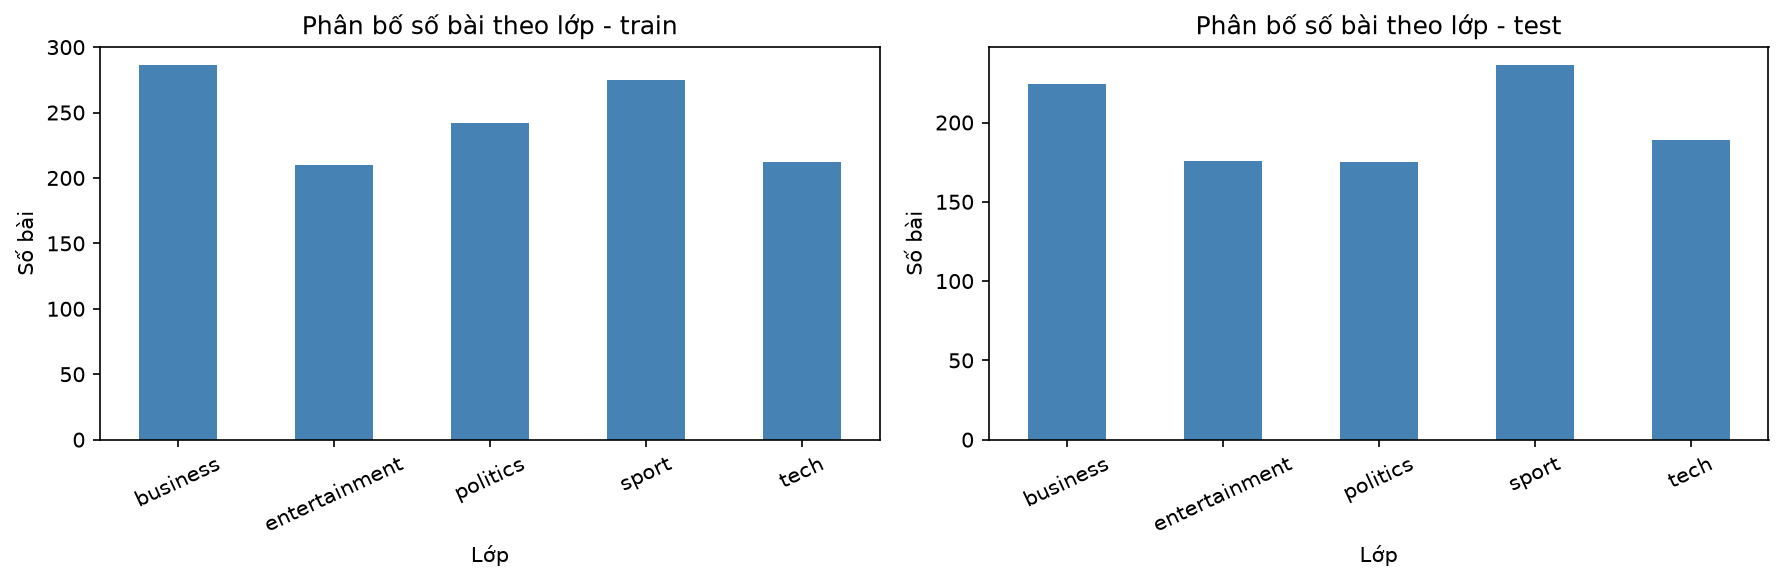
\includegraphics[width=\columnwidth]{report_assets/class_distribution.png}
\caption{Phân bố số bài theo lớp ở hai tập dữ liệu}
\label{fig:class_dist}
\end{figure}

\subsection{Đặc điểm độ dài văn bản}

\begin{table}[!t]
\centering
\caption{Thống kê số từ mỗi bài trước tiền xử lý}
\label{tab:word_stats}
\begin{tabular}{lrr}
\toprule
\textbf{Thống kê} & \textbf{Train} & \textbf{Test} \\
\midrule
Trung bình     & 395,02 & 384,51 \\
Trung vị       & 340    & 334    \\
Độ lệch chuẩn  & 268,24 & 204,67 \\
Nhỏ nhất       & 90     & 116    \\
Lớn nhất       & 4.492  & 3.007  \\
\bottomrule
\end{tabular}
\end{table}

Trung bình lớn hơn trung vị, cùng với sự hiện diện của một số bài dài trên 3.000 từ, cho thấy phân phối độ dài lệch phải. Không có bài nào dưới 20 từ. Xét theo lớp, \textit{tech} có số từ trung bình cao nhất ở cả train (\textbf{516,90}) và test (\textbf{496,66}). \textit{Politics} cũng tương đối dài (\textbf{470,24} và \textbf{448,69}); các lớp còn lại có trung bình khoảng 325--341 từ.

\begin{figure}[!t]
\centering
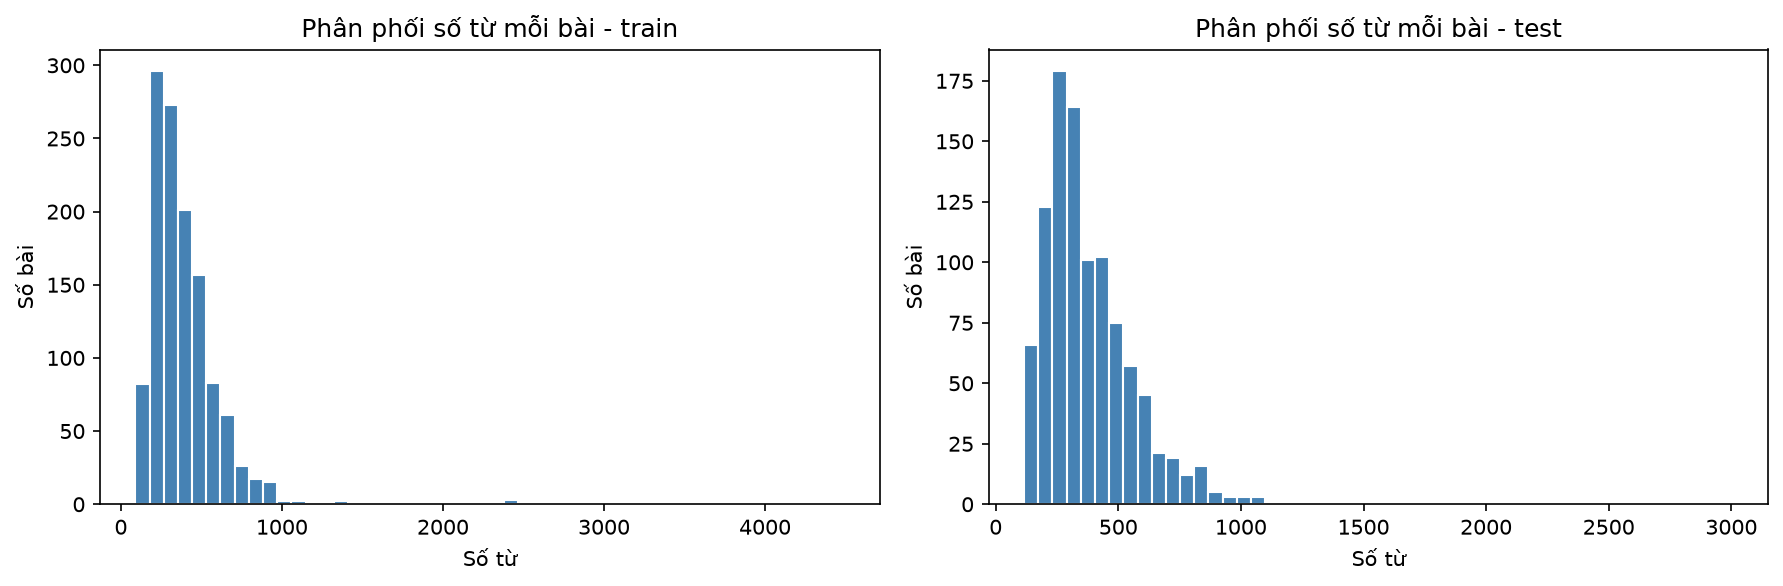
\includegraphics[width=\columnwidth]{report_assets/word_count_hist.png}
\caption{Phân phối số từ mỗi bài}
\label{fig:word_hist}
\end{figure}

\begin{figure}[!t]
\centering
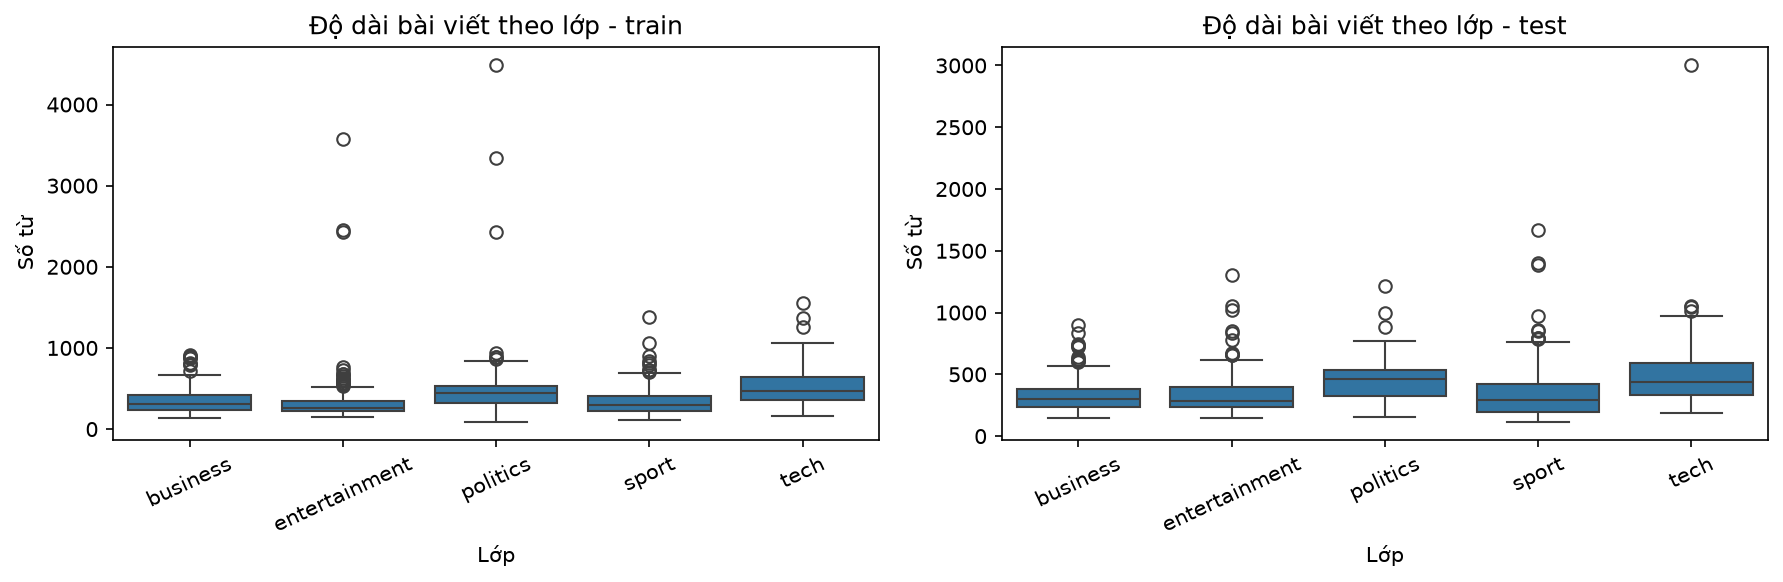
\includegraphics[width=\columnwidth]{report_assets/word_count_boxplot.png}
\caption{Độ dài bài viết theo lớp}
\label{fig:word_boxplot}
\end{figure}

Phép đo bằng tokenizer của \texttt{bert-base-uncased}, tính cả token đặc biệt, cho thấy \textbf{1.014/1.193 bài train (85,00\%)} và \textbf{793/929 bài test (85,36\%)} sau lọc trùng vượt 256 token. Như vậy, \textbf{1.807/2.122 bài (85,16\%)} bị cắt phần cuối khi trích xuất biểu diễn BERT. Tỷ lệ này mô tả phạm vi mất thông tin do giới hạn đầu vào; nó không tự chứng minh tác động nhân quả lên Accuracy.

Phân tích tần suất từ sau loại stop words cho thấy một số tín hiệu từ vựng đặc trưng: \texttt{market}, \texttt{company}, \texttt{economy} ở \textit{business}; \texttt{film}, \texttt{music} ở \textit{entertainment}; \texttt{labour}, \texttt{government}, \texttt{election} ở \textit{politics}; \texttt{game}, \texttt{win}, \texttt{players} ở \textit{sport}; và \texttt{technology}, \texttt{mobile}, \texttt{users} ở \textit{tech}. Từ \texttt{said} xuất hiện nhiều trong mọi lớp nên có ít giá trị phân biệt theo chủ đề.

\subsection{Tiền xử lý và ngăn rò rỉ dữ liệu}

Văn bản dùng cho TF-IDF được chuyển sang chữ thường, loại URL và thẻ HTML, chỉ giữ chữ cái \texttt{a--z} cùng khoảng trắng, rồi chuẩn hóa khoảng trắng. Các bản ghi trùng theo văn bản đã làm sạch được loại riêng trong mỗi tập. Tiếp đó, những bài test có nội dung đã xuất hiện trong train cũng bị loại nhằm tránh đánh giá trên bài mà hệ thống đã thấy khi huấn luyện. Sau mỗi bước, chỉ số hàng được đặt lại để nhãn và đặc trưng giữ đúng thứ tự. BERT sử dụng văn bản gốc và tokenizer đi kèm mô hình.

\begin{table}[!t]
\centering
\caption{Số bài sau từng bước tiền xử lý}
\label{tab:preprocessing}
\begin{tabular}{lrr}
\toprule
\textbf{Bước} & \textbf{Train} & \textbf{Test} \\
\midrule
Ban đầu & 1.225 & 1.000 \\
Sau loại trùng trong từng tập theo văn bản đã làm sạch & 1.193 & 974 \\
Số bài test trùng với train sau bước trên & --- & 45 \\
Đưa vào thí nghiệm & \textbf{1.193} & \textbf{929} \\
\bottomrule
\end{tabular}
\end{table}

Sau xử lý, train có 281 bài \textit{business}, 206 bài \textit{entertainment}, 236 bài \textit{politics}, 274 bài \textit{sport} và 196 bài \textit{tech}. Tập test tương ứng có 221, 163, 167, 228 và 150 bài. Cách lọc này xử lý trùng lặp theo văn bản chuẩn hóa; các bài gần trùng nhưng khác diễn đạt chưa được kiểm tra riêng.

\subsection{Trích xuất đặc trưng}

Với \textbf{TF-IDF}, nghiên cứu sử dụng \texttt{TfidfVectorizer} của scikit-learn \cite{pedregosa2011} với unigram và bigram, \texttt{max\_features=20000}, \texttt{min\_df=2}, \texttt{max\_df=0.95} và \texttt{sublinear\_tf=True}. Bộ vector hóa chỉ được khớp trên train, sau đó áp dụng cho cả train và test. Ma trận đặc trưng thưa có kích thước \textbf{1.193 $\times$ 20.000} và \textbf{929 $\times$ 20.000}, được lưu ở định dạng \texttt{.h5}.

Với \textbf{BERT}, nghiên cứu dùng \texttt{bert-base-uncased} \cite{devlin2019} ở chế độ suy luận, không cập nhật trọng số. Văn bản được cắt hoặc đệm đến tối đa \textbf{256 token}, xử lý theo batch \textbf{16}. Vector của token \texttt{[CLS]} ở lớp cuối được dùng làm biểu diễn 768 chiều; hai ma trận đặc trưng có kích thước \textbf{1.193 $\times$ 768} và \textbf{929 $\times$ 768}, lưu ở định dạng \texttt{float32} (\texttt{.npy}). Cấu hình này khảo sát BERT như một bộ trích xuất đặc trưng cố định, không tương đương với fine-tuning cho tác vụ phân loại BBC News.

\subsection{Mô hình và giao thức đánh giá}

\textbf{Gaussian Naive Bayes} được cài đặt trực tiếp theo quy tắc cực đại hóa log-xác suất hậu nghiệm, với giả định độc lập có điều kiện và phân phối Gauss cho từng đặc trưng. Phương sai được làm mịn bằng \texttt{1e-9} nhân với phương sai lớn nhất trên các đặc trưng; suy luận theo batch để hạn chế dùng bộ nhớ. Trên tập BERT, dự đoán của bản cài đặt trùng với \texttt{sklearn.GaussianNB} ở \textbf{929/929 bài test}. Phép đối chiếu này kiểm tra tính nhất quán của nhãn dự đoán trong cấu hình đã chạy.

\textbf{Decision Tree} sử dụng \texttt{DecisionTreeClassifier} của scikit-learn \cite{pedregosa2011} với tham số mặc định và \texttt{random\_state=42}. Độ sâu cây không bị giới hạn. \textbf{MLP} được cài bằng PyTorch \cite{paszke2019}, gồm sáu khối ẩn kích thước \textbf{1024--512--256--128--64--32}; mỗi khối gồm Linear, ReLU, Dropout (\textbf{0,5}) và BatchNorm1d. Lớp cuối trả về logits cho năm lớp. MLP được huấn luyện \textbf{60 epoch}, mini-batch \textbf{64}, Adam với tốc độ học \textbf{1e-3} và hàm mất mát \texttt{CrossEntropyLoss}.

Mỗi mô hình được huấn luyện riêng trên TF-IDF và BERT, tạo sáu cấu hình. Seed được đặt là \textbf{42}. Tập test 929 bài được dùng để tính Accuracy, Macro Precision, Macro Recall, Macro-F1, Weighted-F1 và ma trận nhầm lẫn. Không có tập validation hoặc tìm kiếm siêu tham số. Lần chạy được báo cáo thực hiện trên \textbf{CPU cục bộ} với BERT embeddings đã được trích xuất trước và lưu trong dự án; do đó, \textbf{thời gian trích xuất BERT từ đầu không được đo}. Hai MLP được huấn luyện đủ 60 epoch trong lần chạy này. Các kết quả số học, đặc biệt của mạng nơ-ron, có thể dao động nhẹ giữa môi trường và lần chạy.

\section{Kết quả thực nghiệm}

\subsection{So sánh tổng thể}

\begin{table*}[!t]
\centering
\caption{Kết quả trên 929 bài test sau lọc trùng, đơn vị \%}
\label{tab:overall_results}
\resizebox{\textwidth}{!}{%
\begin{tabular}{llrrrrr}
\toprule
\textbf{Mô hình} & \textbf{Đặc trưng} & \textbf{Accuracy} & \textbf{Macro Precision} & \textbf{Macro Recall} & \textbf{Macro-F1} & \textbf{Weighted-F1} \\
\midrule
Gaussian Naive Bayes & TF-IDF & 93,86 & 93,69 & 93,70 & 93,44 & 93,89 \\
Gaussian Naive Bayes & BERT   & 91,71 & 91,21 & 91,48 & 91,27 & 91,73 \\
Decision Tree        & TF-IDF & 77,07 & 76,76 & 76,05 & 76,13 & 76,84 \\
Decision Tree        & BERT   & 73,30 & 72,69 & 72,78 & 72,71 & 73,37 \\
\textbf{MLP}         & \textbf{TF-IDF} & \textbf{96,34} & \textbf{96,40} & \textbf{96,10} & \textbf{96,21} & \textbf{96,34} \\
MLP                  & BERT   & 95,37 & 95,12 & 95,47 & 95,25 & 95,37 \\
\bottomrule
\end{tabular}%
}
\end{table*}

\begin{figure}[!t]
\centering
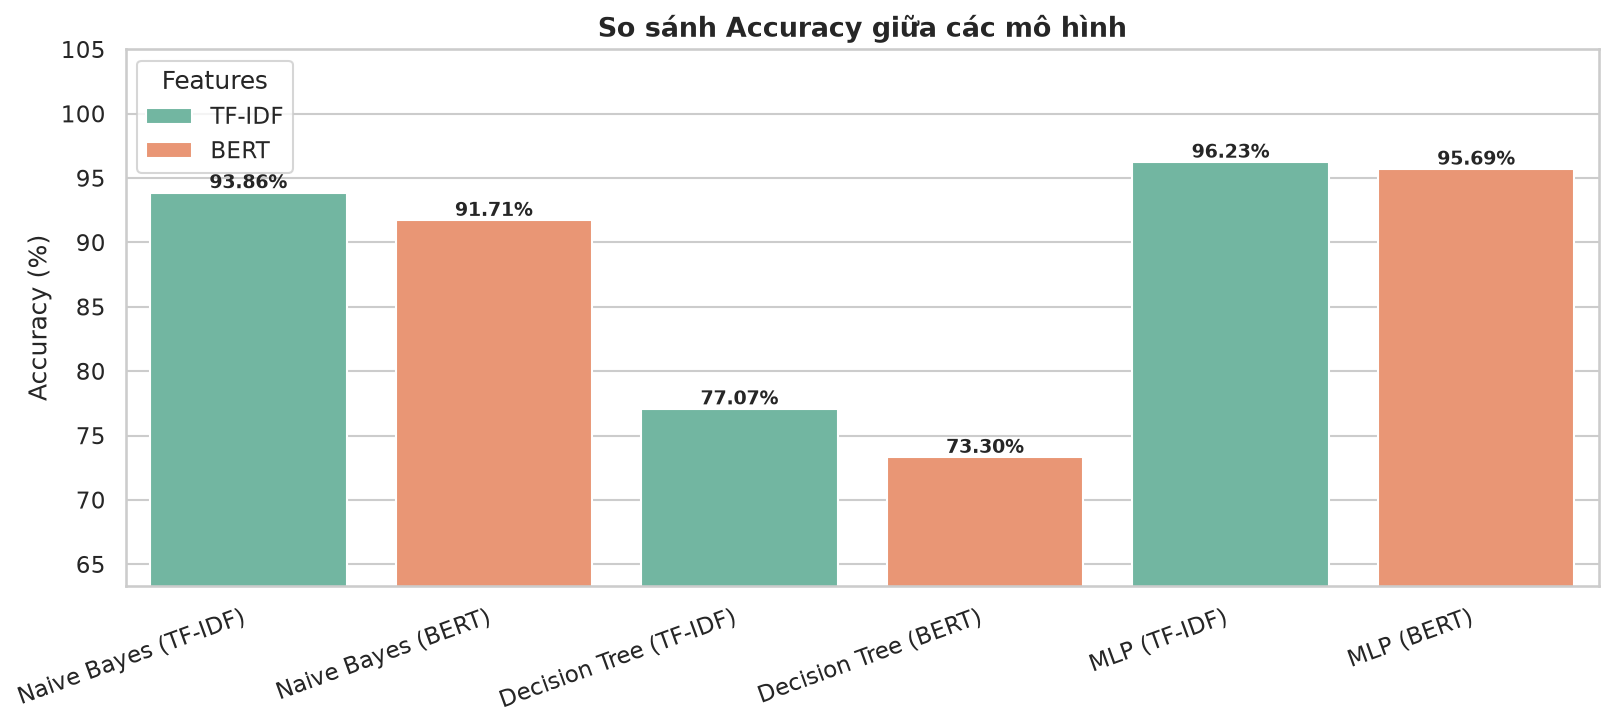
\includegraphics[width=\columnwidth]{report_assets/accuracy_comparison.png}
\caption{Accuracy của sáu cấu hình}
\label{fig:acc_comparison}
\end{figure}

Trong sáu cấu hình, MLP--TF-IDF đạt Accuracy và Macro-F1 cao nhất; Decision Tree--BERT thấp nhất. Chênh lệch giữa Macro-F1 và Weighted-F1 của MLP--TF-IDF là \textbf{0,13 điểm phần trăm}, phù hợp với sự phân bố lớp tương đối đồng đều, dù không loại trừ chênh lệch hiệu quả giữa từng lớp.

\subsection{Kết quả theo lớp và ma trận nhầm lẫn}

\begin{table*}[!t]
\centering
\caption{Precision, Recall và F1 theo lớp của cấu hình tốt nhất và thấp nhất}
\label{tab:per_class}
\small
\setlength{\tabcolsep}{10pt}
\begin{tabular}{l r c c}
\toprule
\textbf{Lớp} & \textbf{Số bài test} & \textbf{MLP--TF-IDF: P / R / F1} & \textbf{Decision Tree--BERT: P / R / F1} \\
\midrule
Tech          & 150 & 0,966 / 0,940 / 0,953 & 0,671 / 0,667 / 0,669 \\
Business      & 221 & 0,942 / 0,955 / 0,948 & 0,722 / 0,729 / 0,725 \\
Sport         & 228 & 0,987 / 0,996 / 0,991 & 0,837 / 0,789 / 0,813 \\
Entertainment & 163 & 0,994 / 0,933 / 0,962 & 0,715 / 0,724 / 0,720 \\
Politics      & 167 & 0,932 / 0,982 / 0,956 & 0,689 / 0,731 / 0,709 \\
\bottomrule
\end{tabular}
\end{table*}

\begin{figure}[!t]
\centering
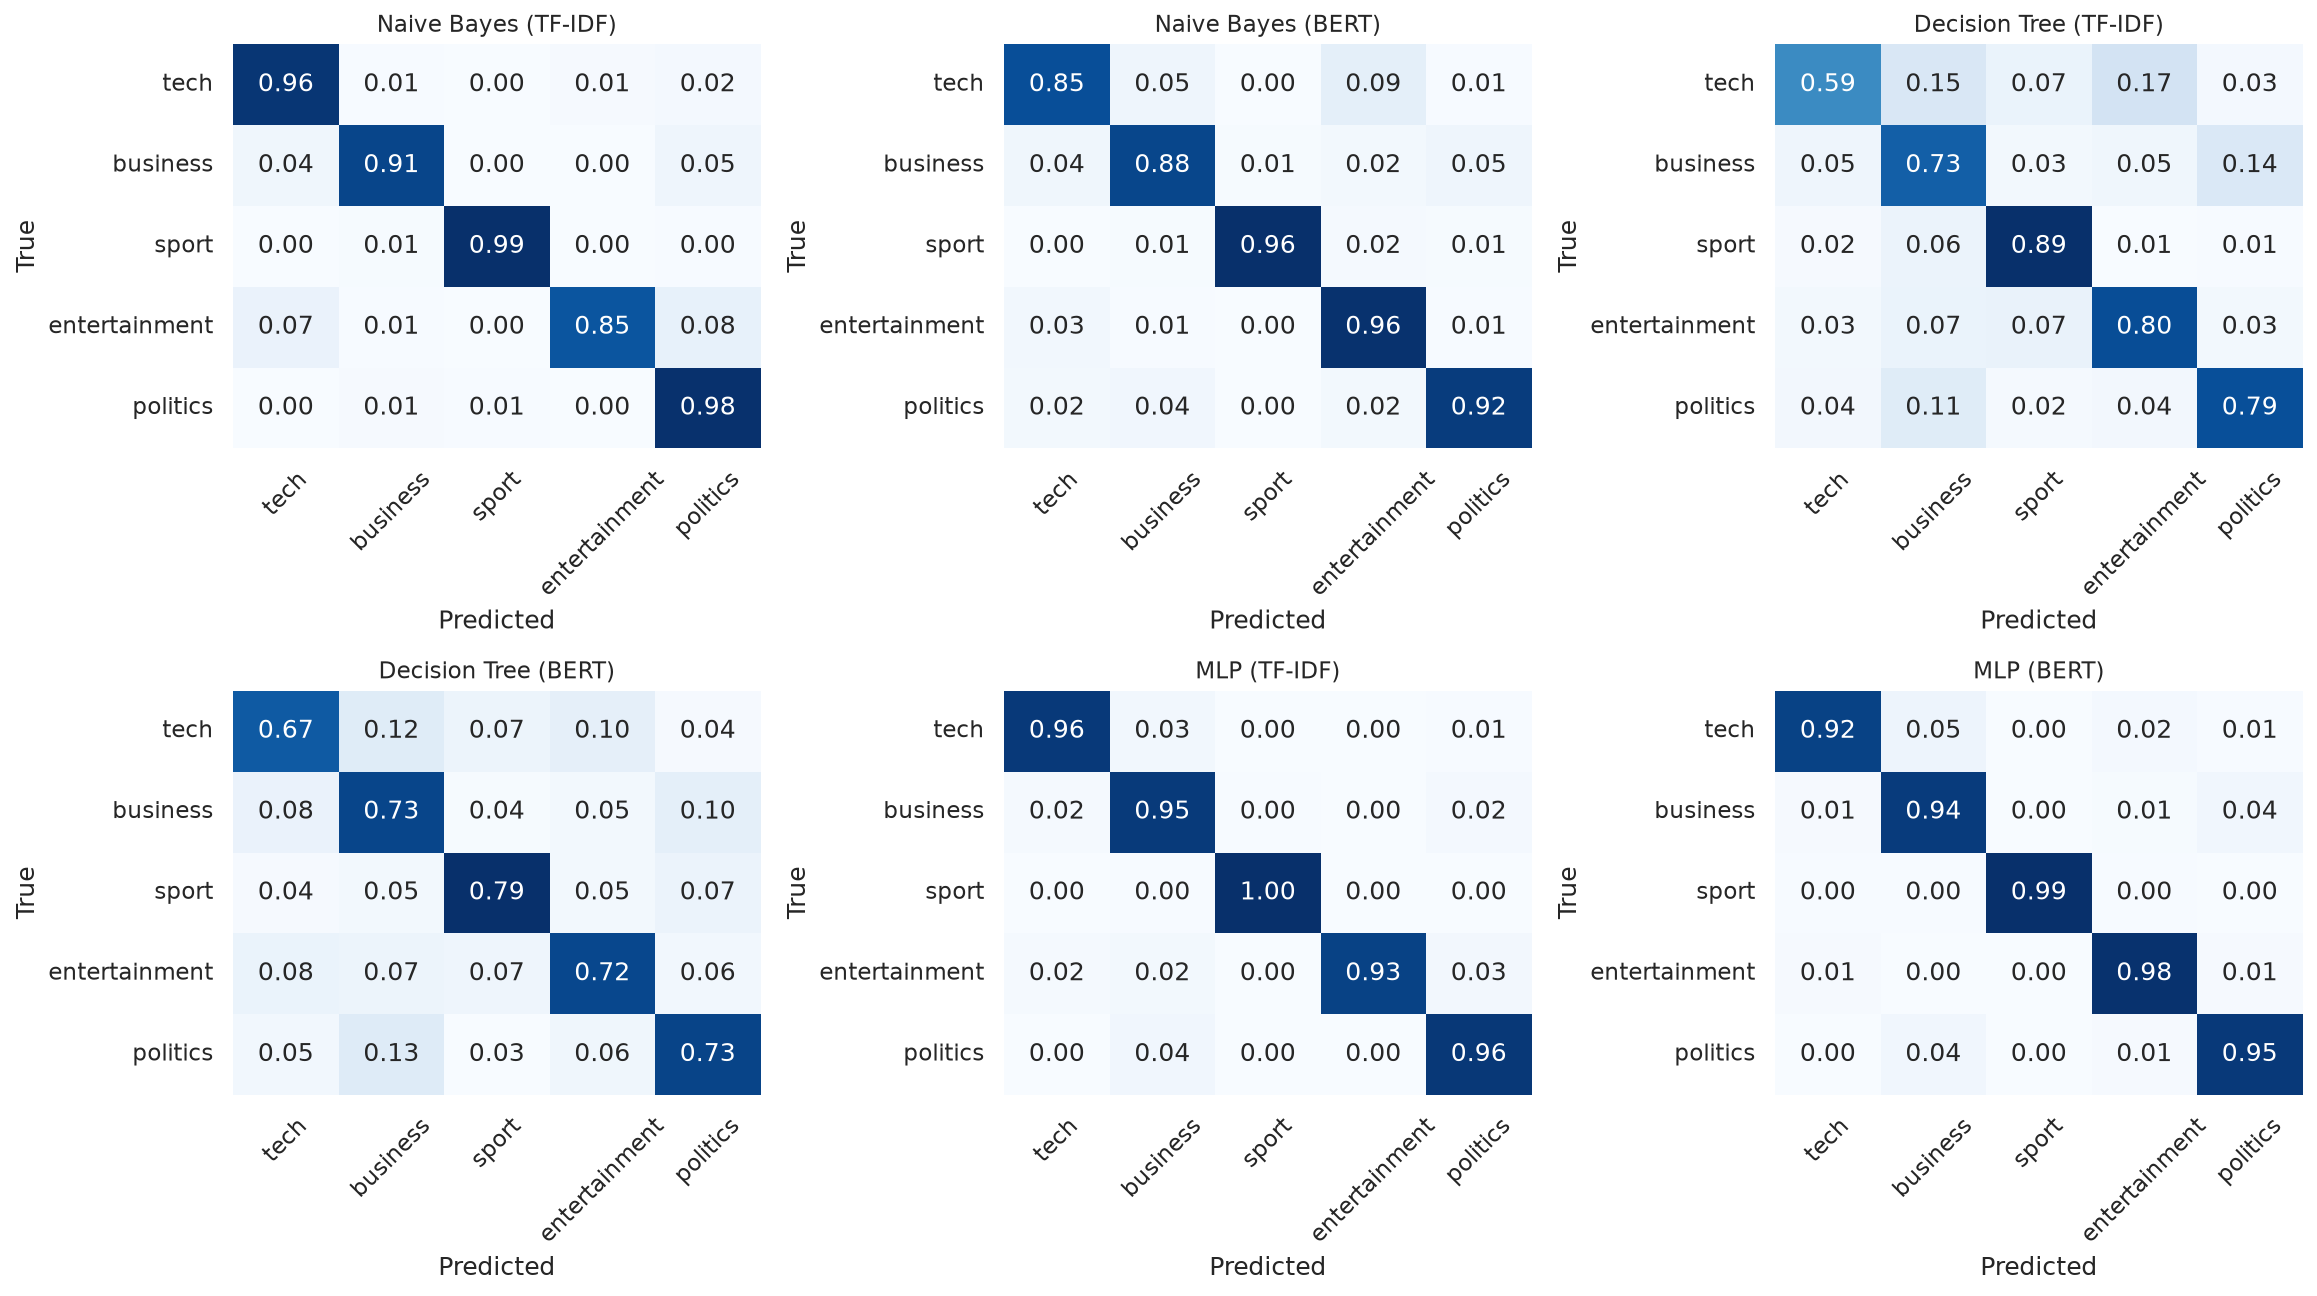
\includegraphics[width=\columnwidth]{report_assets/confusion_matrices.png}
\caption{Ma trận nhầm lẫn chuẩn hóa theo hàng của sáu cấu hình}
\label{fig:confusion_matrices}
\end{figure}

MLP--TF-IDF phân loại đúng \textbf{895/929 bài}. Mô hình này sai nhiều nhất ở các chiều \textit{tech $\rightarrow$ business} (\textbf{6 bài}), \textit{business $\rightarrow$ politics} (\textbf{6 bài}) và \textit{entertainment $\rightarrow$ politics} (\textbf{5 bài}). Decision Tree--BERT đúng \textbf{681/929 bài}; các nhầm lẫn lớn nhất là \textit{business $\rightarrow$ politics} (\textbf{23 bài}) và \textit{politics $\rightarrow$ business} (\textbf{21 bài}).

\subsection{Diễn biến huấn luyện MLP}

\begin{figure}[!t]
\centering
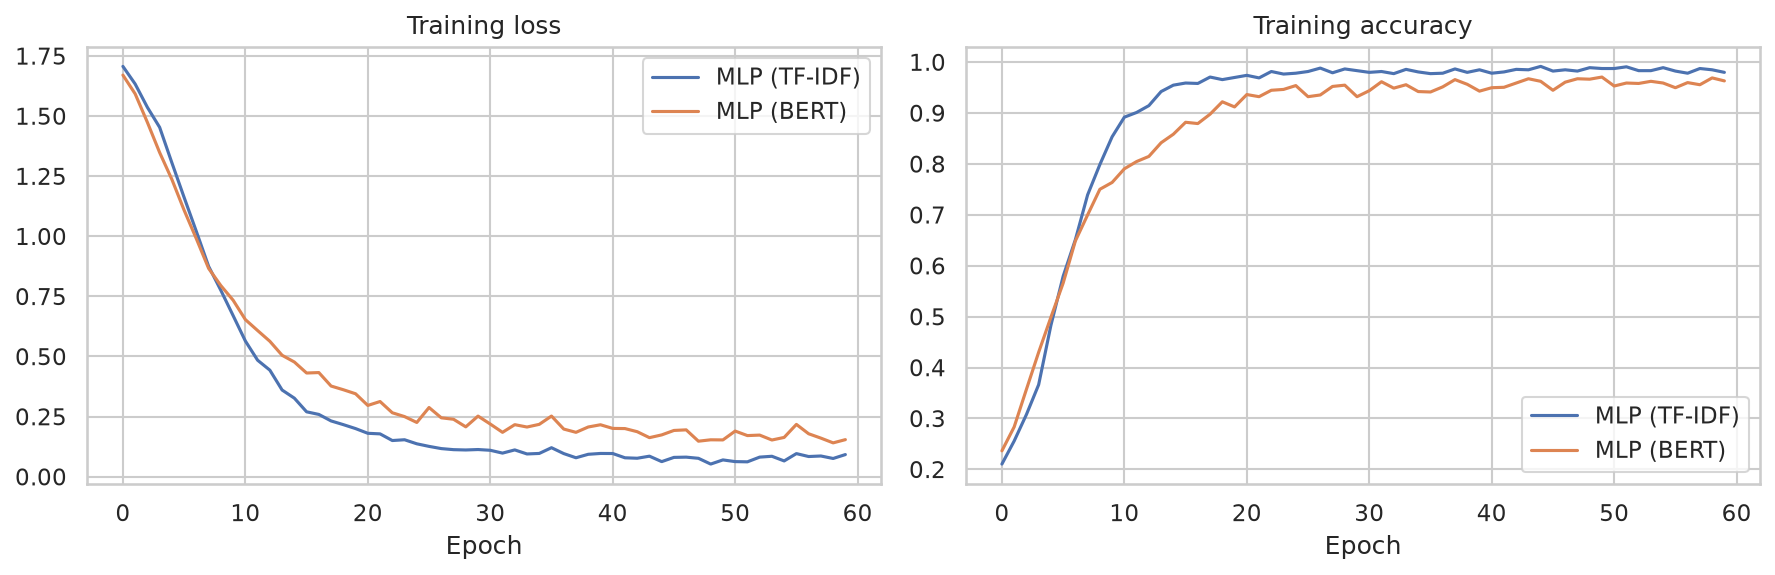
\includegraphics[width=\columnwidth]{report_assets/mlp_training_curves.png}
\caption{Loss và Accuracy trên train trong 60 epoch của hai MLP}
\label{fig:mlp_curves}
\end{figure}

Ở MLP--TF-IDF, loss huấn luyện giảm từ \textbf{1,713} ở epoch đầu xuống \textbf{0,087} ở epoch 60; Accuracy ghi nhận trong huấn luyện tăng từ \textbf{21,88\%} lên \textbf{98,24\%}. Các giá trị tương ứng của MLP--BERT là \textbf{1,684 $\rightarrow$ 0,153} và \textbf{21,96\% $\rightarrow$ 96,73\%}. Ở epoch 20, Accuracy huấn luyện lần lượt là \textbf{94,80\%} và \textbf{93,04\%}. Cả hai đường có dao động; không có đường validation để xác định epoch tối ưu trên dữ liệu chưa thấy.

\section{Thảo luận}

\subsection{Ảnh hưởng của biểu diễn văn bản}

TF-IDF cho Accuracy cao hơn BERT trong cả ba cặp mô hình cùng loại: chênh lệch là 2,15 điểm phần trăm với Naive Bayes, 3,77 điểm với Decision Tree và 0,97 điểm với MLP. Macro-F1 biến động cùng chiều. Tính nhất quán qua ba thuật toán có cơ chế học khác nhau cho thấy ưu thế của TF-IDF không phụ thuộc vào một bộ phân loại cụ thể mà xuất phát từ chất lượng của chính biểu diễn đặc trưng.

Kết quả này phù hợp với bản chất của bài toán. Chủ đề tin tức chủ yếu được xác định bởi các từ và cụm từ đặc trưng như \textit{market}, \textit{film}, \textit{election}, \textit{game} hay \textit{technology} (mục 2.2). TF-IDF giữ lại trực tiếp các tín hiệu này trên toàn bộ văn bản. Ngược lại, cấu hình BERT dùng một vector \texttt{[CLS]} duy nhất từ mô hình chưa tinh chỉnh theo nhãn, đồng thời 85,16\% bài sau lọc trùng vượt quá 256 token nên bị cắt phần cuối. Ba yếu tố gồm pooling bằng \texttt{[CLS]}, giới hạn độ dài đầu vào và việc không fine-tune là những nguyên nhân hợp lý nhất của khoảng cách quan sát được; việc tách riêng đóng góp của từng yếu tố được dành cho nghiên cứu tiếp theo. Kết luận của nghiên cứu áp dụng cho BERT ở vai trò bộ trích xuất đặc trưng cố định, không áp dụng cho BERT đã tinh chỉnh.

Ở cặp MLP, TF-IDF phân loại đúng 895 bài và BERT đúng 886 bài trên 929 bài test, tức chênh lệch 9 bài. Phân tích theo lớp cho thấy chênh lệch này không đồng đều. BERT có recall cao hơn ở \textit{tech} (145/150 so với 141/150) và \textit{entertainment} (155/163 so với 152/163), còn TF-IDF vượt trội rõ nhất ở \textit{business} (211/221 so với 200/221). Lớp \textit{business} vì vậy là nguồn đóng góp chính vào ưu thế tổng thể của TF-IDF.

\subsection{Ảnh hưởng của mô hình phân loại}

\textbf{Gaussian Naive Bayes.} Mô hình đạt 93,86\% Accuracy (sai 57 bài) trên TF-IDF và 91,71\% (sai 77 bài) trên BERT. Dù giả định phân phối Gauss không khớp với đặc trưng thưa của TF-IDF, kết quả vẫn cao. Điều này cho thấy trung bình và phương sai theo từng đặc trưng đã đủ để phân tách các lớp trong bộ dữ liệu này. Accuracy cao không đồng nghĩa với xác suất hậu nghiệm được hiệu chỉnh tốt, nên nếu cần dùng xác suất đầu ra cho các quyết định tiếp theo thì phải đánh giá hiệu chỉnh riêng.

\textbf{Decision Tree.} Đây là mô hình kém nhất trên cả hai biểu diễn, với 213 bài sai (TF-IDF) và 248 bài sai (BERT). Một cây đơn phân tách tuần tự theo từng đặc trưng nên khó nắm bắt thông tin phân loại phân tán trên nhiều từ có tương quan với nhau. Cấu hình không giới hạn độ sâu càng làm tăng khả năng cây khớp với chi tiết riêng của tập huấn luyện.

\textbf{MLP.} Mô hình đứng đầu trên cả hai biểu diễn. Trên TF-IDF, MLP cải thiện 2,48 điểm Accuracy so với Naive Bayes và giảm số bài sai từ 57 xuống 34. Khả năng kết hợp phi tuyến nhiều đặc trưng là cơ chế phù hợp để giải thích mức cải thiện này. Do nghiên cứu không đo thời gian huấn luyện và bộ nhớ, chi phí tính toán đổi lấy mức cải thiện đó chưa được lượng hóa.

\subsection{Phân tích lỗi}

\textbf{MLP--TF-IDF.} Lớp \textit{sport} được nhận diện tốt nhất với recall 227/228 và F1 0,991. Hai lớp có recall thấp nhất là \textit{entertainment} (152/163) và \textit{tech} (141/150). Các nhầm lẫn lớn nhất là \textit{tech $\rightarrow$ business} (6 bài), \textit{business $\rightarrow$ politics} (6 bài) và \textit{entertainment $\rightarrow$ politics} (5 bài). Mô hình do đó phân biệt các chủ đề có từ vựng đặc thù như thể thao tốt hơn các chủ đề có vùng nội dung giao nhau.

Hai ví dụ minh họa cho xu hướng này. Bài ``pc ownership to double by 2010'' (nhãn \textit{tech}) bị dự đoán là \textit{business} vì kết hợp nội dung công nghệ với dự báo thị trường. Bài ``salary scandal in Cameroon'' (nhãn \textit{business}) bị dự đoán là \textit{politics} vì kết hợp vấn đề tài chính với hoạt động của cơ quan nhà nước. Đây là diễn giải dựa trên nội dung văn bản và nhãn dự đoán; việc xác định đặc trưng cụ thể chi phối quyết định của MLP đòi hỏi các phương pháp giải thích mô hình ở mức đặc trưng.

\textbf{Decision Tree--BERT.} Lỗi tập trung ở các cặp chủ đề liền kề: \textit{business $\rightarrow$ politics} (23 bài) và \textit{politics $\rightarrow$ business} (21 bài) cùng chiếm 44/248 lỗi, và có thêm 18 bài \textit{business} bị nhầm thành \textit{tech} cùng 18 bài \textit{tech} bị nhầm thành \textit{business}. Hình mẫu nhầm lẫn của hai mô hình khác nhau về mức độ nhưng giống nhau về cấu trúc: lỗi tập trung ở các cặp \textit{business--politics} và \textit{business--tech}.

\subsection{Độ tin cậy của kết quả}

Với tập test 929 bài, khoảng tin cậy Wilson 95\% cho Accuracy là 94,93--97,37\% đối với MLP--TF-IDF và 93,82--96,55\% đối với MLP--BERT. Hai khoảng này chồng lấp đáng kể, do đó chênh lệch 0,97 điểm giữa hai MLP là nhỏ so với độ bất định của ước lượng. Ngược lại, khoảng cách giữa các nhóm mô hình lớn hơn nhiều: MLP và Naive Bayes đều vượt Decision Tree từ 15 điểm trở lên, và thứ hạng này nằm ngoài phạm vi nhiễu của một lần chạy. Cần lưu ý các khoảng Wilson ở trên mô tả từng tỷ lệ riêng lẻ; để kiểm định hiệu số giữa hai mô hình dự đoán trên cùng tập test, cần dùng kiểm định McNemar hoặc bootstrap ghép cặp trên dự đoán từng bài.

Việc loại 45 bài test trùng với train đã loại bỏ một nguồn rò rỉ dữ liệu trực tiếp. Mô hình tốt nhất được chọn dựa trên điểm test nên ước lượng của nó có thể hơi lạc quan, dù siêu tham số không được tinh chỉnh theo test.

\section{Giới hạn và hướng phát triển}

Nghiên cứu có năm giới hạn: (1) chỉ dùng một bộ dữ liệu tiếng Anh; (2) mỗi cấu hình chỉ chạy một lần với seed 42 nên chưa đo được độ biến thiên theo seed; (3) không có tập validation riêng nên không xác định được epoch tối ưu của MLP; (4) chưa kiểm tra các bài gần trùng khác diễn đạt; (5) chưa tách riêng ảnh hưởng của pooling, độ dài đầu vào và fine-tuning đối với BERT. Vì vậy kết quả mô tả hiệu quả của sáu cấu hình đã khảo sát và chưa là so sánh tổng quát giữa TF-IDF và BERT.

Năm hướng mở rộng được đề xuất:
\begin{enumerate}[leftmargin=*]
    \item Chọn siêu tham số và epoch bằng validation hoặc cross-validation.
    \item Lặp lại thí nghiệm trên nhiều seed và báo cáo khoảng biến thiên.
    \item So sánh \texttt{[CLS]} với mean-pooling, đầu vào dài hơn hoặc chia bài thành nhiều đoạn, và fine-tune BERT.
    \item Bổ sung Logistic Regression hoặc SVM trên TF-IDF làm đối chứng tuyến tính.
    \item Phân tích lỗi mức từng bài, kiểm tra văn bản gần trùng và áp dụng kiểm định McNemar.
\end{enumerate}

\section{Kết luận}

Nghiên cứu so sánh sáu cấu hình học máy trên bài toán phân loại chủ đề BBC News và rút ra ba kết luận chính. Thứ nhất, MLP--TF-IDF đạt kết quả cao nhất với 96,34\% Accuracy và 96,21\% Macro-F1 trên 929 bài test sau loại trùng. Thứ hai, TF-IDF vượt biểu diễn \texttt{[CLS]} của BERT cố định ở cả ba bộ phân loại, với mức chênh từ 0,97 đến 3,77 điểm Accuracy. Thứ ba, mô hình có ảnh hưởng lớn hơn biểu diễn: MLP và Gaussian Naive Bayes (93,86\%) vượt xa Decision Tree (77,07\%), và lỗi của các mô hình tập trung ở các cặp chủ đề có nội dung giao nhau như \textit{business--politics} và \textit{business--tech}. Các kết quả này khẳng định vai trò của tín hiệu từ vựng trong phân loại chủ đề tin tức và cho thấy một biểu diễn đơn giản có thể đạt hiệu quả cao khi phù hợp với tác vụ. Phạm vi áp dụng của kết luận là bộ dữ liệu BBC News và cấu hình BERT cố định đã khảo sát.

\begin{thebibliography}{9}

\bibitem{setfit_bbc}
SetFit, ``BBC News Topic Dataset,'' \textit{Hugging Face Datasets}. Trực tuyến: \url{https://huggingface.co/datasets/SetFit/bbc-news}.

\bibitem{greene2006}
D. Greene và P. Cunningham, ``Practical Solutions to the Problem of Diagonal Dominance in Kernel Document Clustering,'' \textit{Proceedings of ICML}, 2006. DOI: \url{https://doi.org/10.1145/1143844.1143892}.

\bibitem{devlin2019}
J. Devlin, M.-W. Chang, K. Lee và K. Toutanova, ``BERT: Pre-training of Deep Bidirectional Transformers for Language Understanding,'' \textit{Proceedings of NAACL-HLT}, 2019. Trực tuyến: \url{https://aclanthology.org/N19-1423/}.

\bibitem{pedregosa2011}
F. Pedregosa và cộng sự, ``Scikit-learn: Machine Learning in Python,'' \textit{Journal of Machine Learning Research}, tập 12, tr. 2825--2830, 2011. Trực tuyến: \url{https://jmlr.org/papers/v12/pedregosa11a.html}.

\bibitem{paszke2019}
A. Paszke và cộng sự, ``PyTorch: An Imperative Style, High-Performance Deep Learning Library,'' \textit{Advances in Neural Information Processing Systems}, tập 32, 2019. Trực tuyến: \url{https://proceedings.neurips.cc/paper/2019/hash/bdbca288fee7f92f2bfa9f7012727740-Abstract.html}.

\end{thebibliography}

\section*{Tài liệu tái lập}


\begin{itemize}[leftmargin=*]
    \item Notebook độc lập: \texttt{ML\_Assignment\_Standalone.ipynb}.
    \item Bảng kết quả dạng CSV: \texttt{report\_assets/results\_table.csv}.
    \item Các hình trong \texttt{report\_assets/} được tạo từ cùng dữ liệu và lần chạy được mô tả ở mục 2.5.
    \item Mã nguồn dự án của nhóm: \url{https://github.com/AnNguyenGia/ML-assignment}. Đường dẫn Colab công khai chưa được nhóm cung cấp.
\end{itemize}

\end{document}
